\section{Experiments}
\label{sec:experiments}

We compare \tsip~ and \greedy~ on the Iris and Wine datasets \citep{misc_iris_53, misc_wine_109, scikit-learn}, as well as the Ethanol dataset from \citet{Chmiela2018-at, Koelle2022-ju}.
For the latter, a dictionary of interpretable features are evaluated for their ability to parameterize the data manifold through computation of their Jacoban matrices and projection onto estimated tangent spaces (see \citet{Koelle2022-ju} for preprocessing details).
Statistical replicas for Wine and Iris are created by resampling across $P$, while for Ethanol they are created by sampling from data point and their corresponding tangent spaces.
For basis pursuit, we use the SCS interior point solver \citep{ocpb:16} from CVXPY \citep{diamond2016cvxpy, agrawal2018rewriting}, which is able to push sparse values arbitrarily close to 0 \citep{cvxpy_sparse_solution}.
Table \ref{tab:experiments} presents results showing that the $l_c$ accrued by the subset $\widehat S_{G}$ estimated using \greedy~ with objective $l_c$ is higher than that for the subset estimated by \tsip.
We also evaluated second stage \brute~ selection after random selection of $\widehat S_1$ but do not report it since it often lead to catastrophic failure to satisfy the basis pursuit constraint.

\begin{table}[h!]
\tiny
\centering
\begin{tabular}{|c|c|c|c|c|c|c|c|c|c|c|}
\toprule
Name & $D$ & $P$ & $R$ & $c$ & $l_1(X_{.\widehat{S}_{G}})$ & $|\widehat{S}_1|$ & $l_1(X_{.\widehat{S}})$ & $ \thead{ \tiny P_R (l_1(X_{.\widehat{S}_{G}})   \\ > l_1(X_{.\widehat{S}}))}$  & $ \thead{ \tiny P_R (l_1(X_{.\widehat{S}_{G}}) \\ =  l_1(X_{.\widehat{S}}))}$ & $\thead{ \tiny\widehat P(\bar{l}_1(X_{.\widehat{S}_{G}}) \\ > \bar{l}_1(X_{.\widehat{S}}))}$ \\
\midrule
Iris & 4 & 75 & 25 & 1 & 13.8 ± 7.3 & 7 ± 1 & 6.9 ± 1.4 & 0.96 & 0. & 2.4e-05 \\
Wine & 6 & 89 & 25 & 1 & 7.7 ± 0.3 & 13 ± 2 & 7.6 ± 0.3 & 0.64 & 0.16 & 6.3e-04 \\
Ethanol & 2 & 756 & 100 & 1 & 2.6 ± 0.3 & 90 ± 165 & 2.5 ± 0.2 & 0.66 & 0.17 & 2.1e-05 \\
\bottomrule
\end{tabular}
\caption{Experimental parameters and results.
For the Wine dataset, even \brute~ on $\widehat {S}_1$ is prohibitive in $D=13$, and so we truncate our inputs to $D=6$.
For Iris and Wine, $P$ is randomly downsampled by a factor of $2$ to create replicates.
P-values are computed by paired two-sample T-test on  $l_1(X_{.\widehat S})$ and $l_1(X_{.\widehat S_{G}})$.
}
\label{tab:experiments}
\end{table}



\begin{figure}[t]
    \centering
    % Subfigure for Wine dataset
    \begin{subfigure}[b]{0.3\textwidth}
        \centering
        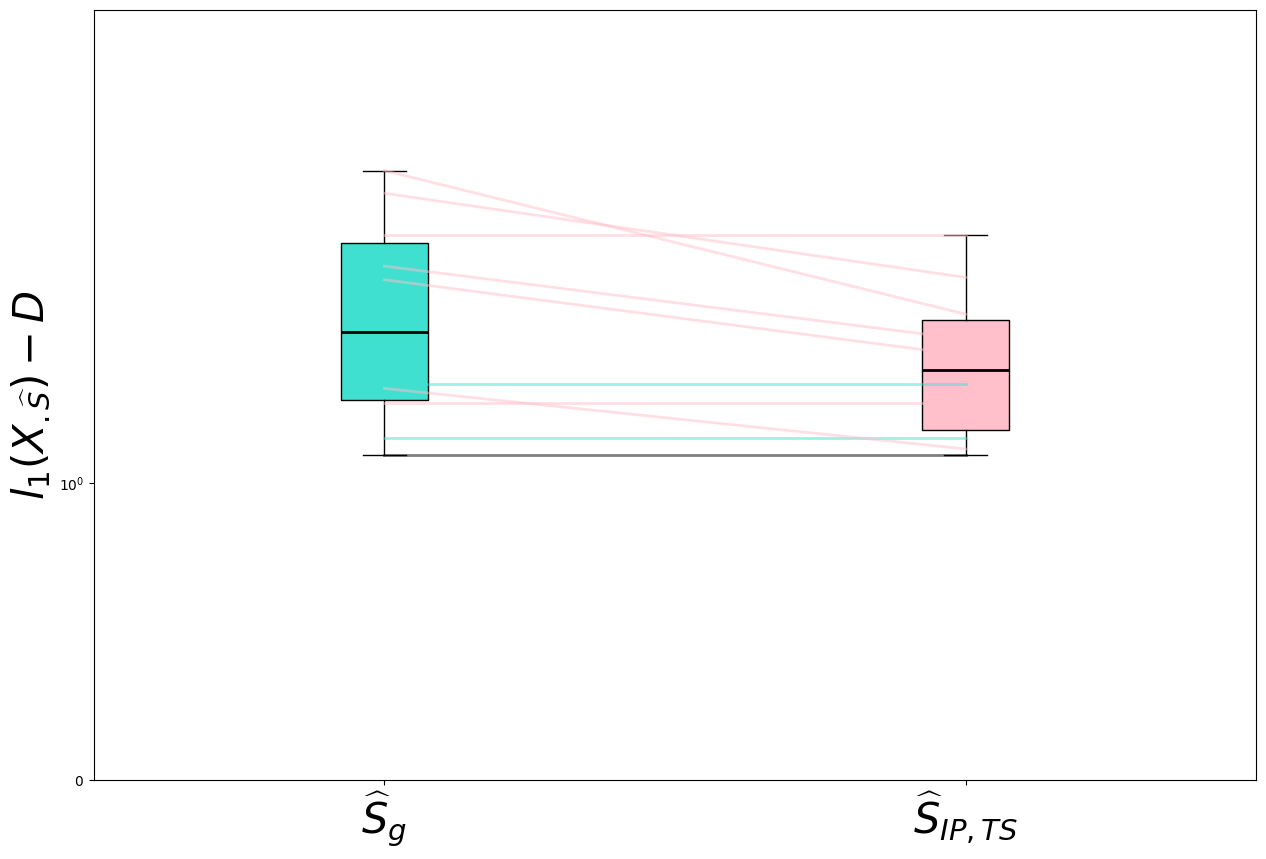
\includegraphics[width=\textwidth]{/Users/samsonkoelle/isometry-pursuit/figures/wine_standardized_0p5_1p0_isometry_losses}
        \caption{Wine Dataset}
        \label{fig:wine_isometry_losses}
    \end{subfigure}
    \hfill
    % Subfigure for Iris dataset
    \begin{subfigure}[b]{0.3\textwidth}
        \centering
        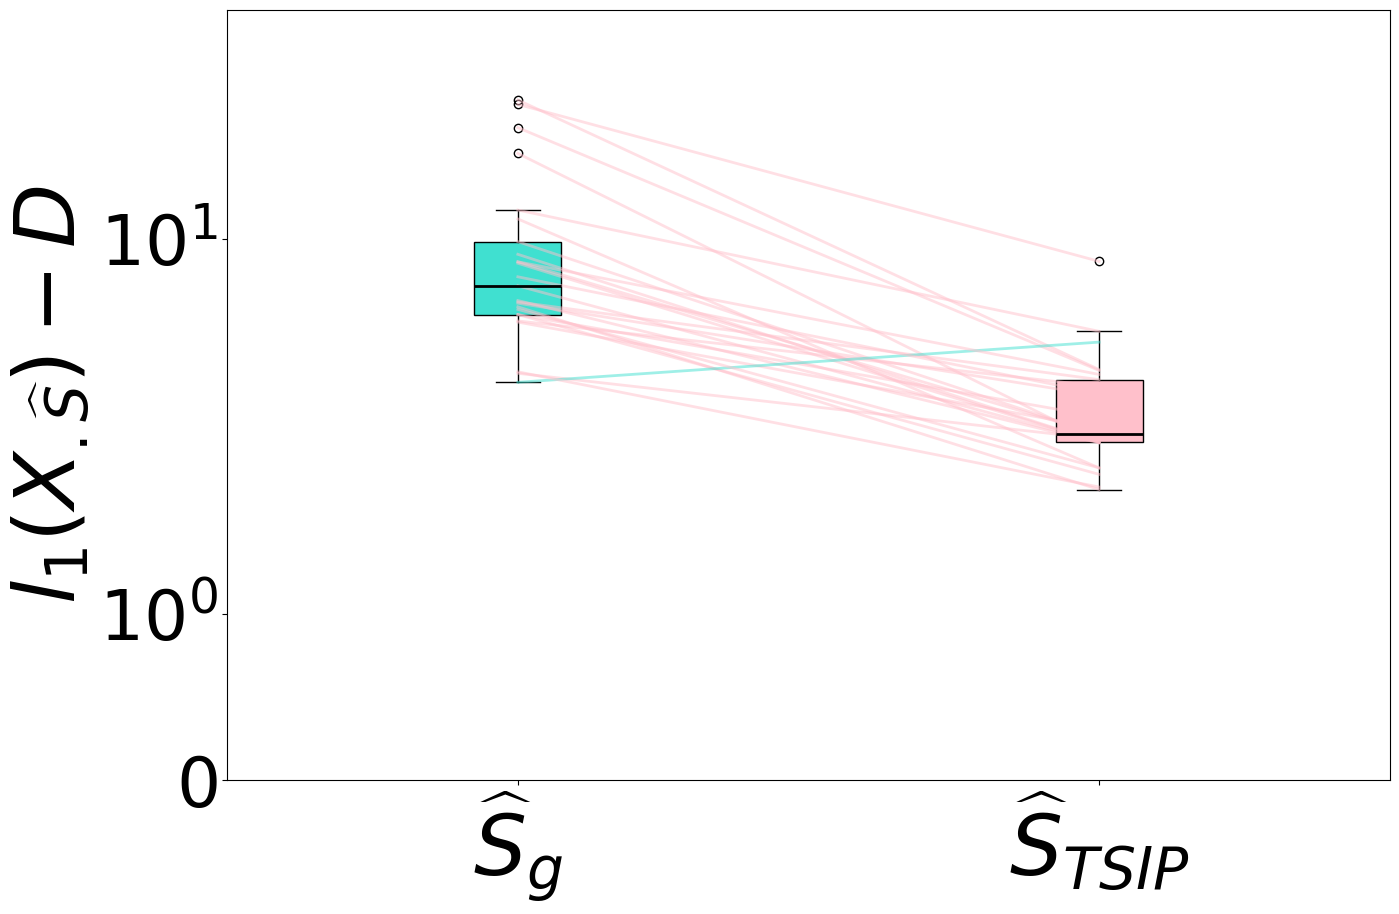
\includegraphics[width=\textwidth]{/Users/samsonkoelle/isometry-pursuit/figures/iris_standardized_0p5_1p0_isometry_losses}
        \caption{Iris Dataset}
        \label{fig:iris_isometry_losses}
    \end{subfigure}
    \hfill
    % Subfigure for Ethanol dataset
    \begin{subfigure}[b]{0.3\textwidth}
        \centering
        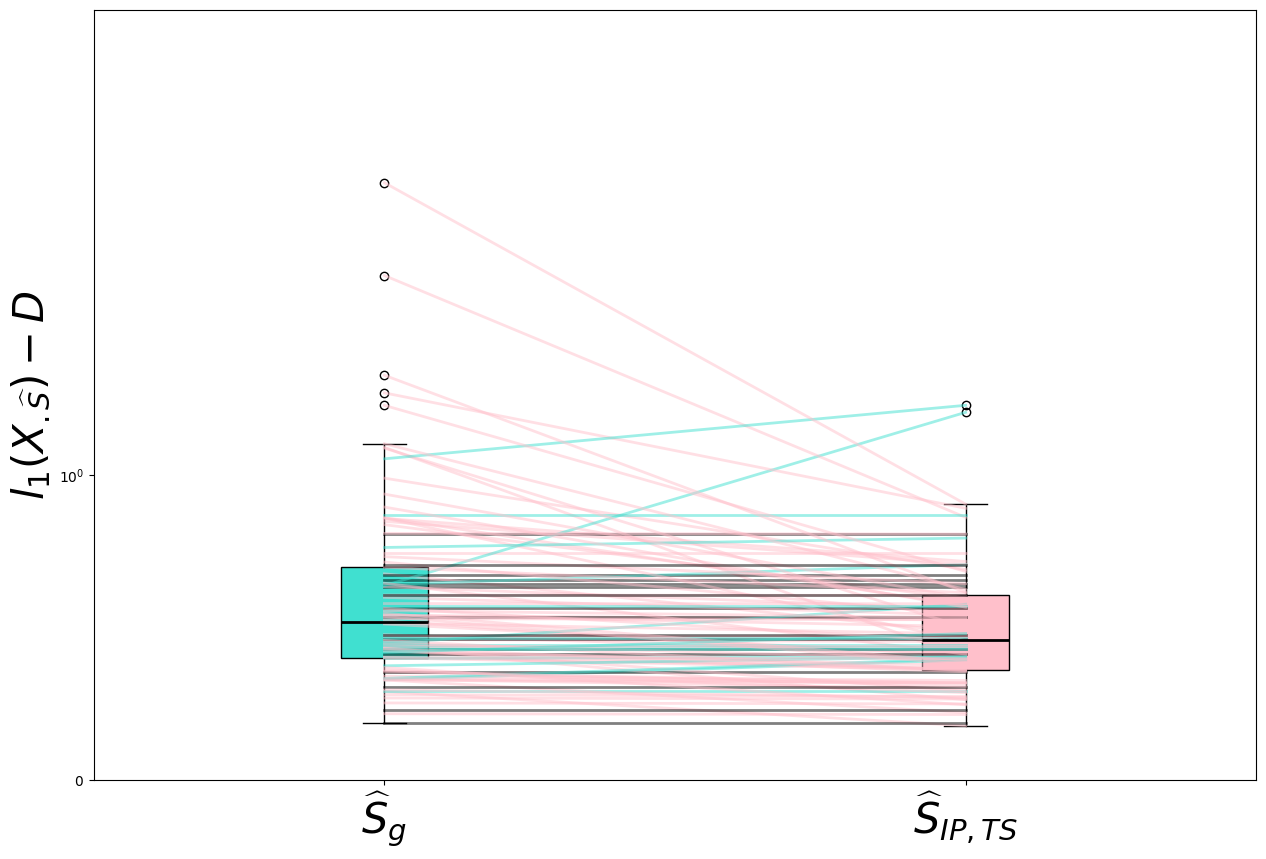
\includegraphics[width=\textwidth]{/Users/samsonkoelle/isometry-pursuit/figures/ethanol_isometry_losses}
        \caption{Ethanol Dataset}
        \label{fig:ethanol_isometry_losses}
    \end{subfigure}
    \caption{Isometry Loss Comparisons for Wine, Iris, and Ethanol Datasets}
    \label{fig:isometry_losses}
\end{figure}



% TODO (Sam): remove mathcal on S
